Dans l’espace rapporté à un repère orthonormé $\Rijk$, on considère les points : 

$A$ de coordonnées $(2;0;0)$, $B$ de coordonnées $(0;3;0)$ et $C$ de coordonnées $(0;0;1)$.

\begin{center}
	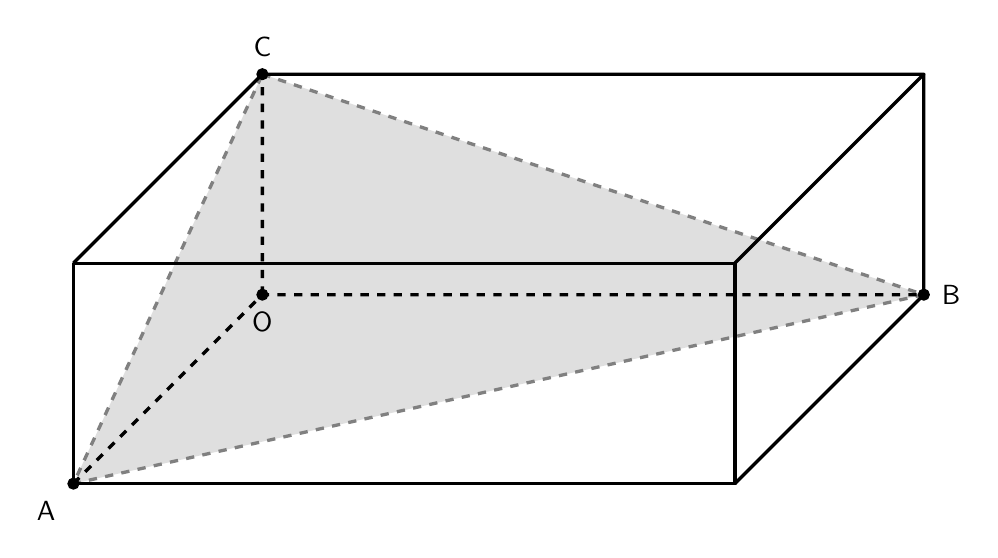
\begin{tikzpicture}[line join=round]
		\coordinate (O) at (0,0) ; \coordinate (B) at (8.4,0) ;
		\coordinate (C) at (0,2.8) ; \coordinate (A) at (-2.4,-2.4) ;
		\coordinate (E) at (-2.4,0.4) ; \coordinate (F) at (6,0.4) ;
		\coordinate (D) at (6,-2.4) ; \coordinate (G) at (8.4,2.8) ;
		\filldraw[very thick,dashed,gray,fill=lightgray!50] (C) -- (B) -- (A) -- cycle ;
		\draw[very thick] (A) -- (E) -- (F) -- (D) --cycle ;
		\draw[very thick] (E) -- (C) -- (G) -- (F) ;
		\draw[very thick] (D) -- (B) -- (G) ;
		\draw[very thick,dashed] (A) -- (O) -- (B) (O) -- (C) ;
		\foreach \Point/\Pos in {O/below,A/below left,B/right,C/above} \filldraw (\Point) circle[radius=2pt] node[\Pos=3pt,font=\sffamily] {\Point} ;
	\end{tikzpicture}
\end{center}

L’objectif de cet exercice est de calculer l’aire du triangle $ABC$.

\begin{enumerate}
	\item 
	\begin{enumerate}
		\item Montrer que le vecteur $\vect{n} \coordve{3}{2}{6}$ est normal au plan $(ABC)$.
		\item En déduire qu’une équation cartésienne du plan $(ABC)$ est : $3x+2y+6z-6=0$.
	\end{enumerate}
	\item On note $d$ la droite passant par $O$ et orthogonale au plan $(ABC)$.
	\begin{enumerate}
		\item Déterminer une représentation paramétrique de la droite $d$.
		\item Montrer que la droite $d$ coupe le plan $(ABC)$ au point $H$ de coordonnées $\left( \dfrac{18}{49};\dfrac{12}{49};\dfrac{36}{49} \right)$. 
		\item Calculer la distance $OH$.
	\end{enumerate}
	\item On rappelle que le volume d’une pyramide est donné par : $\mathcal{V}=\dfrac13 \mathcal{B}h$, où $\mathcal{B}$ est l’aire d’une base et $h$ est la hauteur de la pyramide correspondant à cette base.
	
	\smallskip
	
	En calculant de deux façons différentes le volume de la pyramide $OABC$, déterminer l’aire du triangle $ABC$.
\end{enumerate}

